\documentclass[lettersize,journal]{IEEEtran}

\usepackage{amsmath,amsfonts,amssymb}
\usepackage{array}
\usepackage[caption=false,font=normalsize,labelfont=sf,textfont=sf]{subfig}
\usepackage{textcomp}
\usepackage{stfloats}
\usepackage{url}
\usepackage{graphicx}
\usepackage{cite}
\usepackage{xcolor}
\usepackage{balance}
\usepackage{booktabs}
\usepackage{tabularx}
\usepackage{ragged2e}
\usepackage{float}
\usepackage{algorithm}
\usepackage{algpseudocode}
\usepackage{tikz}
\usetikzlibrary{positioning,arrows.meta,fit,calc,shapes.geometric,decorations.pathreplacing}



\newcolumntype{Y}{>{\RaggedRight\arraybackslash}X}
\newcolumntype{P}[1]{>{\RaggedRight\arraybackslash}p{#1}}

\newcommand{\status}[1]{\textbf{#1}}

\begin{document}
	\title{Graphical User Interface and PC--ESP32 Communication Standard for the SOFIA Vision System}

	\author{
		Marco Heimdal Castro Magaña, Alejandro Amador Franco, Karen Alejandra Guevara Vasquez, María Alicia Vela Contreras, Juan Pablo Contreras Quiñones,
		Jorge A. Lizarraga, Luis E. González-Jiménez, Luis F. Luque-Vega

		\thanks{The authors are affiliated with the Instituto Tecnológico de Estudios Superiores de Occidente (ITESO), Tlaquepaque, Jalisco, Mexico.}
	}


	\markboth{Laboratory for the Development of Technological Solutions}
	{Graphical User Interface and PC--ESP32 Communication Standard for SOFIA}

	\maketitle


	\begin{abstract}
		The SOFIA modular kinetic surface uses an external computer vision system that recognizes five human gestures to drive its actuators. This work presents the graphical user interface (GUI) that displays the live video and the detection result, and the wireless communication standard that transmits the recognized gestures from the host PC to the ESP32 master controller. The GUI was implemented with PySide6 and separates the interface, the video processing, and the Bluetooth Low Energy (BLE) link into independent threads, so that the detection can be started, paused, resumed, and stopped without blocking user interaction. The communication standard defines a frame of 5 to 19 bytes with a sequence number and a CRC-8 checksum, five commands, positive and negative acknowledgements, six error codes, and rules for retransmission, duplicate rejection, and link supervision. An ESP32 firmware was developed to receive, validate, and acknowledge the frames, and to map each gesture to a distinct motion pattern on one two-degree-of-freedom SOFIA unit. In addition, a Webots simulation of the complete 16-unit array was integrated with the GUI: a simulated master controller receives the same frames over a local TCP socket, validates and acknowledges them with the same rules as the firmware, and drives the 16 simulated units, while an overhead virtual camera streams its images to the GUI through an independent channel. The GUI can send its results to the simulation, to the physical ESP32, or to both at the same time, operating the simulation as a digital twin of the robot. The implementation was verified through software tests, a simulation of the firmware, and the Webots simulation, and a preliminary functional test on the physical ESP32 and one unit confirmed the BLE link and the servo motion; a quantitative characterization of the hardware remains as the next step.
	\end{abstract}

	\begin{IEEEkeywords}
		Graphical user interface, multithreading, Bluetooth Low Energy, communication protocol, ESP32, gesture recognition, modular robotics, Webots, digital twin.
	\end{IEEEkeywords}


	\section{Introduction}
	\label{sec:intro}

	\IEEEPARstart{S}{OFIA} is a modular robotic installation composed of 16 mechatronic units arranged in a honeycomb configuration, where each unit provides two rotational degrees of freedom actuated by servomotors \cite{sofia_architecture}. Interaction with the user is achieved through an external computer vision system that recognizes five gestures (INICIO, RECARGAR, ESCUDO, ATAQUE, and FIN) using MediaPipe Pose Landmarker and Hand Landmarker \cite{lugaresi2019mediapipe}, and that also tracks the position of the user's hand.

	Before this work, the vision system operated as an independent prototype: the result was shown in an OpenCV window controlled through the keyboard, and the recognized gestures were not transmitted to the embedded controller. Integrating the vision system with the robot requires two elements. First, a GUI that allows an operator to visualize the detection and control the processing without freezing the interface, since landmark detection takes tens of milliseconds per frame. Second, a communication standard that delivers the recognized gestures to the ESP32 master controller \cite{esp32c3} reliably over a wireless link.

	Testing these elements on the robot requires the complete array of 16 units, which is not always available, and a fault in the communication or in a motion pattern can only be observed after loading the firmware. For this reason, a simulation of SOFIA in Webots \cite{webots} was also connected to the GUI, using the same communication standard as the physical robot.

This work addresses five activities: (i) the design of the GUI architecture and wireframes, including the justification of the framework; (ii) the integration of the detection result into the GUI using threads; (iii) the implementation of controls to start, stop, and resume the detection; (iv) the design and implementation of the PC--ESP32 communication standard; and (v) the integration of a Webots simulation of the 16-unit array that receives the same frames and can run alongside the physical robot as a digital twin. The remainder of this paper is organized as follows. Section~\ref{sec:gui} presents the GUI design, Section~\ref{sec:impl} describes its implementation, Section~\ref{sec:protocol} defines the communication standard, Section~\ref{sec:esp32} presents the ESP32 firmware, Section~\ref{sec:webots} describes the Webots simulation and the digital twin, Section~\ref{sec:verification} reports the verification, and Section~\ref{sec:conclusions} concludes the work.


	\section{GUI Architecture and Design}
	\label{sec:gui}

	\subsection{Framework Selection}

	The main requirement of the GUI is to display video at the camera frame rate while the landmark detection runs, without blocking the interaction with the user. The alternatives considered are compared in Table~\ref{tab:framework}.

	\begin{table}[!t]
		\centering
		\caption{Comparison of GUI Frameworks}
		\label{tab:framework}
		\scriptsize

		\setlength{\tabcolsep}{2pt}
		\renewcommand{\arraystretch}{1.05}

		\begin{tabularx}{\columnwidth}{@{}P{2.2cm} Y Y Y@{}}
			\toprule
			Criterion & \textbf{PySide6 (Qt)} & Tkinter / CustomTkinter & Web (Flask + browser)\\
			\midrule
			Threads integrated with the GUI & Native (\texttt{QThread}, thread-safe signals) & Manual (queues and polling) & Separate server process\\
			Video display & Direct (\texttt{QImage}) & Through PIL conversion & MJPEG streaming\\
			Synchronization primitives & \texttt{QMutex}, \texttt{QWaitCondition} & Not included & Not included\\
			Styling & Style sheets (QSS) & Basic / moderate & Extensive\\
			License & LGPL & PSF / MIT & --\\
			\bottomrule
		\end{tabularx}
	\end{table}

	PySide6, the official Python binding of Qt \cite{pyside6}, was selected because it provides the mechanisms required by the problem: \texttt{QThread} to move the processing out of the interface thread, signals and slots to transfer data between threads safely, and \texttt{QMutex} with \texttt{QWaitCondition} to pause a thread without busy waiting. In addition, frames captured by OpenCV can be converted directly into a \texttt{QImage} without intermediate libraries, and its LGPL license is compatible with an academic project.

	\subsection{Software Architecture}

	The application is organized in modules with a single responsibility each, as shown in Fig.~\ref{fig:architecture} and Table~\ref{tab:modules}. The detection logic is encapsulated in a pipeline shared by the GUI and by the original keyboard-based application, so that both use exactly the same implementation.

	\begin{figure}[!t]
		\centering
		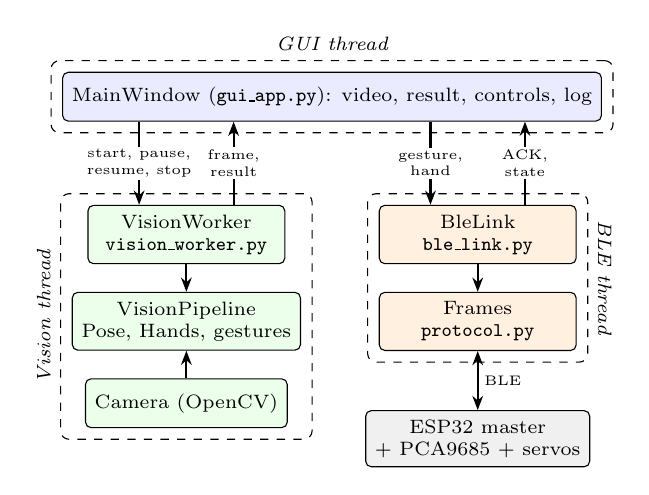
\begin{tikzpicture}[
			font=\scriptsize,
			box/.style={draw, rounded corners=2pt, align=center, minimum width=2.5cm, minimum height=0.62cm, fill=white},
			thread/.style={draw, dashed, rounded corners=3pt, inner sep=4pt},
			arr/.style={-{Stealth[length=1.8mm]}, thick},
			lbl/.style={font=\tiny, align=center, fill=white, inner sep=1pt}
			]
			% GUI thread
			\node[box, fill=blue!8, minimum width=6.6cm] (gui) at (0,0) {MainWindow (\texttt{gui\_app.py}): video, result, controls, log};
			% Vision thread
			\node[box, fill=green!8] (worker) at (-1.85,-1.75) {VisionWorker\\\texttt{vision\_worker.py}};
			\node[box, fill=green!8, below=0.35cm of worker] (pipe) {VisionPipeline\\Pose, Hands, gestures};
			\node[box, fill=green!8, below=0.35cm of pipe] (cam) {Camera (OpenCV)};
			% BLE thread
			\node[box, fill=orange!12] (ble) at (1.85,-1.75) {BleLink\\\texttt{ble\_link.py}};
			\node[box, fill=orange!12, below=0.35cm of ble] (proto) {Frames\\\texttt{protocol.py}};
			\node[box, fill=gray!12, below=0.75cm of proto] (esp) {ESP32 master\\+ PCA9685 + servos};
			
			\node[thread, fit=(gui), label={[font=\scriptsize\itshape]above:GUI thread}] {};
			\node[thread, fit=(worker)(pipe)(cam), label={[font=\scriptsize\itshape]left:\rotatebox{90}{Vision thread}}] {};
			\node[thread, fit=(ble)(proto), label={[font=\scriptsize\itshape]right:\rotatebox{-90}{BLE thread}}] {};
			
			% GUI <-> vision
			\draw[arr] ([xshift=-6mm]gui.south -| worker) -- node[lbl]{start, pause,\\resume, stop} ([xshift=-6mm]worker.north);
			\draw[arr] ([xshift=6mm]worker.north) -- node[lbl]{frame,\\result} ([xshift=6mm]gui.south -| worker);
			% GUI <-> BLE
			\draw[arr] ([xshift=-6mm]gui.south -| ble) -- node[lbl]{gesture,\\hand} ([xshift=-6mm]ble.north);
			\draw[arr] ([xshift=6mm]ble.north) -- node[lbl]{ACK,\\state} ([xshift=6mm]gui.south -| ble);
			% internal
			\draw[arr] (worker) -- (pipe);
			\draw[arr] (cam) -- (pipe);
			\draw[arr] (ble) -- (proto);
			\draw[{Stealth[length=1.8mm]}-{Stealth[length=1.8mm]}, thick] (proto) -- node[lbl, right=1pt]{BLE} (esp);
		\end{tikzpicture}
		\caption{Software architecture of the GUI. Each dashed region runs in its own thread.}
		\label{fig:architecture}
	\end{figure}

	\begin{table}[!t]
		\centering
		\caption{Main Software Components}
		\label{tab:modules}
		\scriptsize

		\setlength{\tabcolsep}{2pt}
		\renewcommand{\arraystretch}{1.05}

		\begin{tabularx}{\columnwidth}{@{}P{3.3cm} Y@{}}
			\toprule
			Module & Responsibility\\
			\midrule
			\texttt{gui\_app.py} & Window, controls, and visualization; it does not process video\\
			\texttt{vision\_worker.py} & Thread that reads the camera and runs the pipeline; implements pause, resume, and stop\\
			\texttt{vision\_pipeline.py} & Processes one frame according to the active mode (game or hand tracking)\\
			\texttt{gesture\_recognition.py} & Decides the recognized gesture from the landmarks\\
			\texttt{hand\_tracker.py} & Hand position in a Cartesian plane centered on the image\\
			\texttt{ble\_link.py} & BLE connection, transmission with acknowledgement, and retransmission\\
			\texttt{protocol.py} & Construction and validation of frames\\
			\texttt{sim\_link.py} & Same logic as \texttt{ble\_link.py} over a TCP socket to the Webots simulation\\
			\texttt{sim\_camera.py} & Thread that receives the images of the virtual camera of Webots\\
			\bottomrule
		\end{tabularx}
	\end{table}

	\subsection{Threading Model}

	The application uses three threads (Table~\ref{tab:threads}). The GUI thread only draws widgets and handles user events. The vision thread captures frames and runs MediaPipe, which requires approximately 20 to 40~ms per frame. The BLE thread runs an \texttt{asyncio} event loop for the Bleak library \cite{bleak}, since scanning, connecting, and waiting for acknowledgements may take from milliseconds to seconds.

	\begin{table}[!t]
		\centering
		\caption{Threads of the Application}
		\label{tab:threads}
		\scriptsize

		\setlength{\tabcolsep}{2pt}
		\renewcommand{\arraystretch}{1.05}

		\begin{tabularx}{\columnwidth}{@{}P{1.4cm} Y Y@{}}
			\toprule
			Thread & Task & Communication with the GUI\\
			\midrule
			GUI & Draws the window and handles clicks & --\\
			Vision & Camera capture and landmark detection & Qt signals (queued connections); commands protected by \texttt{QMutex}\\
			BLE & Scanning, connection, transmission, and acknowledgement wait & Coroutines scheduled in the event loop from the GUI thread; results through Qt signals\\
			\bottomrule
		\end{tabularx}
	\end{table}

	Communication from the vision thread to the GUI uses Qt signals, which Qt delivers in the receiving thread through queued connections. In the opposite direction, the GUI calls methods of the worker that modify state variables protected by a \texttt{QMutex}. In this way, no widget is accessed outside the GUI thread and no shared variable is accessed without synchronization.

	\subsection{Wireframe and Layout}

	The main window is shown in Fig.~\ref{fig:wireframe}. The video occupies the left side, since it is the main element of the interface, while a fixed-width column on the right groups the controls in the order in which they are used: detection control, mode, result, ESP32 connection, and event log.

	\begin{figure*}[!t]
		\centering
		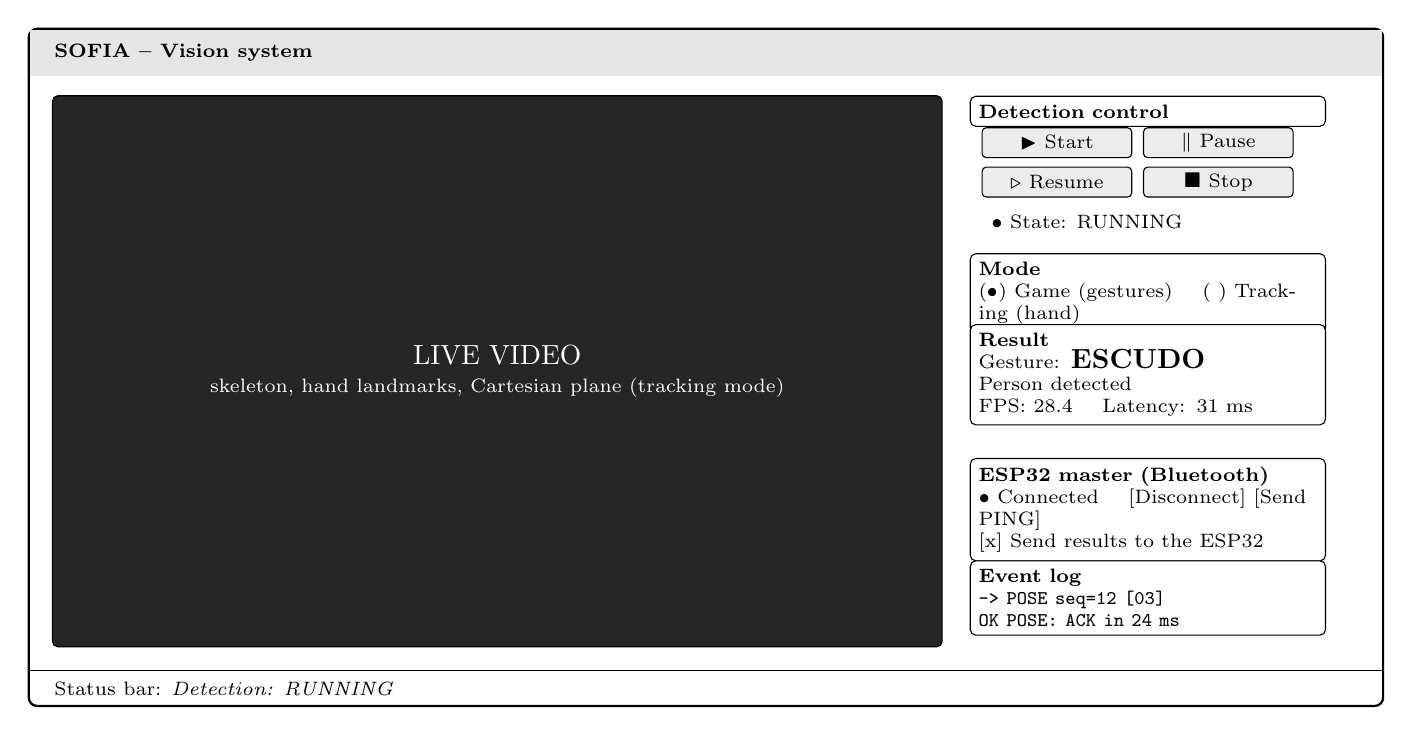
\begin{tikzpicture}[
			font=\scriptsize,
			panel/.style={draw, rounded corners=2pt, fill=white, align=left, inner sep=3pt, text width=4.3cm},
			btn/.style={draw, rounded corners=1.5pt, fill=gray!15, minimum width=1.9cm, minimum height=0.38cm, inner sep=1pt}
			]
			\draw[thick, rounded corners=3pt] (0,0) rectangle (17.2,8.6);
			\fill[gray!20] (0.02,8.0) rectangle (17.18,8.58);
			\node[anchor=west] at (0.2,8.3) {\textbf{SOFIA -- Vision system}};
			\draw (0,0.45) -- (17.2,0.45);
			\node[anchor=west] at (0.2,0.22) {Status bar: \emph{Detection: RUNNING}};

			\draw[fill=black!85, rounded corners=2pt] (0.3,0.75) rectangle (11.6,7.75);
			\node[white, align=center] at (5.95,4.25) {\normalsize LIVE VIDEO\\[2pt] skeleton, hand landmarks, Cartesian plane (tracking mode)};

			\node[panel, anchor=north west] (ctrl) at (11.95,7.75) {\textbf{Detection control}\\[2.15cm]};
			\node[btn, anchor=north west] at (12.1,7.35) {$\blacktriangleright$ Start};
			\node[btn, anchor=north west] at (14.15,7.35) {$\|$ Pause};
			\node[btn, anchor=north west] at (12.1,6.85) {$\triangleright$ Resume};
			\node[btn, anchor=north west] at (14.15,6.85) {$\blacksquare$ Stop};
			\node[anchor=north west] at (12.1,6.35) {$\bullet$ State: RUNNING};

			\node[panel, anchor=north west] at (11.95,5.75) {\textbf{Mode}\\ (\textbullet) Game (gestures) \quad ( ) Tracking (hand)};
			\node[panel, anchor=north west] at (11.95,4.85) {\textbf{Result}\\ Gesture: {\normalsize\textbf{ESCUDO}}\\ Person detected\\ FPS: 28.4 \quad Latency: 31 ms};
			\node[panel, anchor=north west] at (11.95,3.15) {\textbf{ESP32 master (Bluetooth)}\\ $\bullet$ Connected \quad [Disconnect] [Send PING]\\ {[x]} Send results to the ESP32};
			\node[panel, anchor=north west] at (11.95,1.85) {\textbf{Event log}\\ \texttt{-> POSE seq=12 [03]}\\ \texttt{OK POSE: ACK in 24 ms}};
		\end{tikzpicture}
		\caption{Wireframe of the main window. The right column keeps every control visible without covering the video.}
		\label{fig:wireframe}
	\end{figure*}

	The interaction flow is as follows: the operator optionally connects to the ESP32 and sends a PING to verify the link, selects the mode, and starts the detection. During the detection, the operator can pause, resume, or stop the processing, and change the mode, which is applied from the next frame. The design decisions are summarized in Table~\ref{tab:decisions}.

	\begin{table}[!t]
		\centering
		\caption{Design Decisions of the GUI}
		\label{tab:decisions}
		\scriptsize

		\setlength{\tabcolsep}{2pt}
		\renewcommand{\arraystretch}{1.05}

		\begin{tabularx}{\columnwidth}{@{}P{2.6cm} Y@{}}
			\toprule
			Decision & Justification\\
			\midrule
			Large video, fixed right column & The video is the main element; the controls remain visible\\
			Grouped panels & Each group corresponds to one task, ordered by the usage flow\\
			Buttons enabled by state & Prevents invalid actions, such as resuming a stopped process\\
			Color state indicators & The state of the thread and of the link is recognized at a glance\\
			Large result label & The gesture can be read at a distance from the camera\\
			Event log & Shows every frame sent and its acknowledgement; useful as evidence and for debugging\\
			``Send results'' option & Allows testing the vision system without moving the robot\\
			Shared detection pipeline & The GUI runs the same code that was evaluated in the keyboard application\\
			\bottomrule
		\end{tabularx}
	\end{table}


	\section{Detection Visualization and Controls}
	\label{sec:impl}

	\subsection{Processing Thread}

	The processing is performed by \texttt{VisionWorker}, a subclass of \texttt{QThread}. The camera and the MediaPipe models are created inside the thread that uses them, and each processed frame is sent to the GUI as a \texttt{QImage} together with the detection result and the frame rate. The loop of the thread is summarized in Algorithm~\ref{alg:worker}.

	\begin{algorithm}[!t]
		\caption{Processing loop of the vision thread}
		\label{alg:worker}
		\begin{algorithmic}[1]
			\Require Camera index, initial mode
			\State Open camera and load Pose and Hand Landmarker
			\State Emit state \textsc{Running}
			\Loop
			\State Lock mutex
			\If{\textit{paused} \textbf{and} \textit{running}}
			\State Emit state \textsc{Paused}
			\While{\textit{paused} \textbf{and} \textit{running}}
			\State Wait on condition (no CPU use)
			\EndWhile
			\EndIf
			\State $m \gets$ requested mode; unlock mutex
			\If{\textbf{not} \textit{running}} \textbf{break} \EndIf
			\State Capture frame; process it with the pipeline in mode $m$
			\State Emit frame, result, FPS, and latency to the GUI
			\EndLoop
			\State Release camera and models; emit state \textsc{Stopped}
		\end{algorithmic}
	\end{algorithm}

	\subsection{Detection Controls}

	Each control produces a specific effect on the processing thread, as described in Table~\ref{tab:controls}, and the resulting state transitions are shown in Fig.~\ref{fig:states}. The pause is implemented with a \texttt{QWaitCondition}: the thread is blocked without consuming CPU until \texttt{resume()} or \texttt{stop()} wakes it up. The buttons are enabled according to the current state, so only valid transitions can be requested.

	\begin{table}[!t]
		\centering
		\caption{Effect of Each Control on the Processing Thread}
		\label{tab:controls}
		\scriptsize

		\setlength{\tabcolsep}{2pt}
		\renewcommand{\arraystretch}{1.05}

		\begin{tabularx}{\columnwidth}{@{}P{1.2cm} Y P{1.5cm}@{}}
			\toprule
			Control & Effect on the thread & Camera\\
			\midrule
			Start & Creates the worker and calls \texttt{start()}; the camera and models are loaded inside the thread & Opened\\
			Pause & Sets \textit{paused}; the thread blocks on \texttt{QWaitCondition} at the next iteration & Open (video frozen)\\
			Resume & Clears \textit{paused} and calls \texttt{wakeAll()}; the loop continues & Open\\
			Stop & Clears \textit{running} and calls \texttt{wakeAll()}; the loop ends and resources are released; a STOP frame is sent to the ESP32 & Closed\\
			\bottomrule
		\end{tabularx}
	\end{table}

	\begin{figure}[!t]
		\centering
		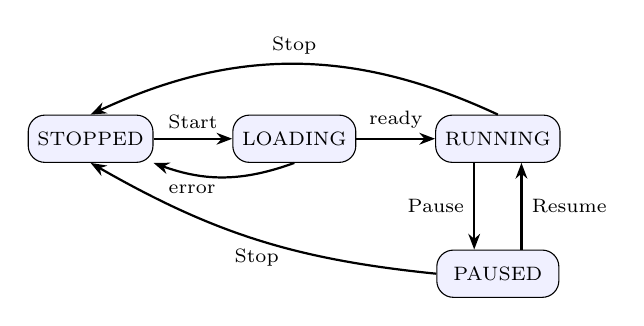
\begin{tikzpicture}[
			font=\scriptsize,
			st/.style={draw, rounded corners=6pt, minimum width=1.55cm, minimum height=0.6cm, fill=blue!6},
			arr/.style={-{Stealth[length=2mm]}, thick}
			]
			\node[st] (stopped) {STOPPED};
			\node[st, right=1.0cm of stopped] (loading) {LOADING};
			\node[st, right=1.0cm of loading] (running) {RUNNING};
			\node[st, below=1.1cm of running] (paused) {PAUSED};

			\draw[arr] (stopped) -- node[above]{Start} (loading);
			\draw[arr] (loading) -- node[above]{ready} (running);
			\draw[arr] ([xshift=-3mm]running.south) -- node[left]{Pause} ([xshift=-3mm]paused.north);
			\draw[arr] ([xshift=3mm]paused.north) -- node[right]{Resume} ([xshift=3mm]running.north |- running.south);
			\draw[arr] (running.north) to[bend right=25] node[above]{Stop} (stopped.north);
			\draw[arr] (paused.west) to[bend left=12] node[below]{Stop} (stopped.south);
			\draw[arr] (loading.south) to[bend left=20] node[below left=-1pt]{error} (stopped.south east);
		\end{tikzpicture}
		\caption{States of the processing thread and the controls that produce each transition.}
		\label{fig:states}
	\end{figure}

	\subsection{Visualization of the Result}

	In game mode, the result panel shows the recognized gesture and whether a person is detected. In tracking mode, Pose detection and gesture recognition are disabled; the panel shows the position of the hand in a Cartesian plane whose origin is the center of the image, normalized to $[-1,1]$ on each axis, together with the magnitude and angle of the vector from the origin to the hand. The video shows the landmarks and, in tracking mode, the plane and the vector.


	\section{Communication Standard}
	\label{sec:protocol}

	\subsection{Link Layer}

	The ESP32-C3 supports Bluetooth Low Energy but not Bluetooth Classic \cite{esp32c3}; therefore, the link uses BLE \cite{bt_core} with the Nordic UART Service (NUS) profile \cite{nordic_nus}, a de facto standard that can also be tested with generic BLE applications. The ESP32 acts as a peripheral (GATT server) and the PC as a central (GATT client). The parameters are listed in Table~\ref{tab:ble}. Each BLE write carries exactly one complete frame, and the longest frame (19 bytes) fits in the default BLE payload of 20 bytes, so no MTU negotiation is required.

	\begin{table}[!t]
		\centering
		\caption{BLE Link Parameters}
		\label{tab:ble}
		\scriptsize

		\setlength{\tabcolsep}{2pt}
		\renewcommand{\arraystretch}{1.05}

		\begin{tabularx}{\columnwidth}{@{}P{2.4cm} Y@{}}
			\toprule
			Parameter & Value\\
			\midrule
			Advertised name & \texttt{SOFIA-ESP32}\\
			Service & \texttt{6E400001-B5A3-F393-E0A9-E50E24DCCA9E}\\
			RX (PC $\rightarrow$ ESP32) & \texttt{6E400002-\ldots}, write without response\\
			TX (ESP32 $\rightarrow$ PC) & \texttt{6E400003-\ldots}, notify\\
			Maximum frame & 19 bytes (one BLE write)\\
			\bottomrule
		\end{tabularx}
	\end{table}

	\subsection{Frame Structure}

	The frame structure is shown in Fig.~\ref{fig:frame} and its fields are described in Table~\ref{tab:fields}. Multi-byte integers are transmitted in little-endian order.

	\begin{figure}[!t]
		\centering
		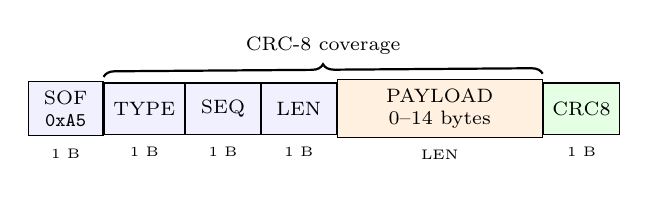
\begin{tikzpicture}[
			font=\scriptsize,
			f/.style={draw, minimum height=0.65cm, align=center, fill=blue!6}
			]
			\node[f, minimum width=0.95cm] (sof) {SOF\\\texttt{0xA5}};
			\node[f, minimum width=0.95cm, right=0pt of sof] (type) {TYPE};
			\node[f, minimum width=0.95cm, right=0pt of type] (seq) {SEQ};
			\node[f, minimum width=0.95cm, right=0pt of seq] (len) {LEN};
			\node[f, minimum width=2.6cm, right=0pt of len, fill=orange!12] (pay) {PAYLOAD\\0--14 bytes};
			\node[f, minimum width=0.95cm, right=0pt of pay, fill=green!10] (crc) {CRC8};
			\foreach \n/\t in {sof/1 B, type/1 B, seq/1 B, len/1 B, pay/LEN, crc/1 B}{
				\node[below=1pt of \n, font=\tiny] {\t};
			}
			\draw[decorate, decoration={brace, amplitude=4pt}, thick] ([yshift=2pt]type.north west) -- node[above=4pt]{CRC-8 coverage} ([yshift=2pt]pay.north east);
		\end{tikzpicture}
		\caption{Frame structure of the communication standard.}
		\label{fig:frame}
	\end{figure}

	\begin{table}[!t]
		\centering
		\caption{Frame Fields}
		\label{tab:fields}
		\scriptsize

		\setlength{\tabcolsep}{2pt}
		\renewcommand{\arraystretch}{1.05}

		\begin{tabularx}{\columnwidth}{@{}P{1.4cm} P{0.9cm} Y@{}}
			\toprule
			Field & Size & Description\\
			\midrule
			SOF & 1 B & Start of frame, always \texttt{0xA5}\\
			TYPE & 1 B & Message type (Table~\ref{tab:types})\\
			SEQ & 1 B & Sequence number 0--255; each side keeps its own counter\\
			LEN & 1 B & Payload length, 0--14\\
			PAYLOAD & 0--14 B & Message data\\
			CRC8 & 1 B & CRC-8 over TYPE, SEQ, LEN, and PAYLOAD\\
			\bottomrule
		\end{tabularx}
	\end{table}

	The checksum is a CRC-8 with polynomial \texttt{0x07} ($x^8+x^2+x+1$), initial value \texttt{0x00}, no reflection, and no final XOR. With these parameters, $\text{CRC8}(\text{``123456789''}) = \texttt{0xF4}$, which is used as a check value for any implementation.

	\subsection{Commands and Payloads}

	The message types are listed in Table~\ref{tab:types}. The POSE command carries the identifier of the recognized gesture (1~INICIO, 2~RECARGAR, 3~ESCUDO, 4~ATAQUE, 5~FIN) and is sent only when a new gesture appears. The TRACK command carries the hand position (Table~\ref{tab:track}) normalized with respect to the image, so it does not depend on the camera resolution. Since TRACK is a continuous stream in which the most recent value supersedes the previous ones, it does not require acknowledgement.

	\begin{table}[!t]
		\centering
		\caption{Message Types}
		\label{tab:types}
		\scriptsize

		\setlength{\tabcolsep}{2pt}
		\renewcommand{\arraystretch}{1.05}

		\begin{tabularx}{\columnwidth}{@{}P{0.8cm} P{1.0cm} P{1.5cm} P{0.9cm} Y@{}}
			\toprule
			TYPE & Name & Direction & Payload & ACK\\
			\midrule
			\texttt{0x00} & POSE & PC $\rightarrow$ ESP32 & 1 B & Yes\\
			\texttt{0x01} & TRACK & PC $\rightarrow$ ESP32 & 9 B & No\\
			\texttt{0x02} & PING & PC $\rightarrow$ ESP32 & 0 B & Yes\\
			\texttt{0x03} & MODE & PC $\rightarrow$ ESP32 & 1 B & Yes\\
			\texttt{0x04} & STOP & PC $\rightarrow$ ESP32 & 0 B & Yes\\
			\texttt{0x80} & ACK & ESP32 $\rightarrow$ PC & 2 B & --\\
			\texttt{0x81} & NACK & ESP32 $\rightarrow$ PC & 3 B & --\\
			\bottomrule
		\end{tabularx}
	\end{table}

	\begin{table}[!t]
		\centering
		\caption{TRACK Payload}
		\label{tab:track}
		\scriptsize

		\setlength{\tabcolsep}{2pt}
		\renewcommand{\arraystretch}{1.05}

		\begin{tabularx}{\columnwidth}{@{}P{0.9cm} P{1.0cm} P{0.8cm} Y@{}}
			\toprule
			Bytes & Field & Type & Encoding and range\\
			\midrule
			0 & hand & u8 & 0 left, 1 right\\
			1--2 & $x$ & i16 & $x_\text{norm}\times1000$, $-1000$ to $1000$\\
			3--4 & $y$ & i16 & $y_\text{norm}\times1000$, $-1000$ to $1000$\\
			5--6 & $|v|$ & u16 & $|v|_\text{norm}\times1000$, 0 to 1415\\
			7--8 & angle & u16 & degrees $\times10$, 0 to 3599\\
			\bottomrule
		\end{tabularx}
	\end{table}

	The PING command has no payload and is used both as the test command and as a heartbeat. The MODE command informs the active mode (0~game, 1~test, 2~tracking), and the STOP command requests the ESP32 to enter a safe state.

	\subsection{Acknowledgements and Error Codes}

	The ESP32 answers each valid command that requires confirmation with an ACK whose payload contains the type and sequence number of the confirmed command. Invalid frames are answered with a NACK that contains the received type, the received sequence number, and an error code (Table~\ref{tab:errors}). The ESP32 validates each frame in the order length, SOF, LEN, CRC, type, and payload, and reports the first error found.

	\begin{table}[!t]
		\centering
		\caption{Error Codes}
		\label{tab:errors}
		\scriptsize

		\setlength{\tabcolsep}{2pt}
		\renewcommand{\arraystretch}{1.05}

		\begin{tabularx}{\columnwidth}{@{}P{0.75cm} P{2.55cm} Y P{0.85cm}@{}}
			\toprule
			Code & Name & Cause & PC retries\\
			\midrule
			\texttt{0x01} & \texttt{ERR\_SOF} & First byte is not \texttt{0xA5} & No\\
			\texttt{0x02} & \texttt{ERR\_LENGTH} & Frame size or LEN invalid & No\\
			\texttt{0x03} & \texttt{ERR\_CRC} & Checksum mismatch & Yes\\
			\texttt{0x04} & \texttt{ERR\_UNKNOWN\_TYPE} & Undefined TYPE & No\\
			\texttt{0x05} & \texttt{ERR\_PAYLOAD} & Payload size or values out of range & No\\
			\texttt{0x06} & \texttt{ERR\_BUSY} & Reception queue full & Yes\\
			\bottomrule
		\end{tabularx}
	\end{table}

	\subsection{Communication Rules}

	The rules of Table~\ref{tab:rules} make the communication robust against lost frames, corrupted frames, and loss of the link. Fig.~\ref{fig:sequence} illustrates the case in which an acknowledgement is lost: the PC retransmits the command with the same sequence number, and the ESP32 recognizes it as a duplicate, so the unit does not execute the same motion twice.

	\begin{table}[!t]
		\centering
		\caption{Communication Rules}
		\label{tab:rules}
		\scriptsize

		\setlength{\tabcolsep}{2pt}
		\renewcommand{\arraystretch}{1.05}

		\begin{tabularx}{\columnwidth}{@{}P{0.55cm} Y@{}}
			\toprule
			Rule & Description\\
			\midrule
			R1 & Commands with ACK are sent one at a time (stop-and-wait)\\
			R2 & ACK timeout of 300~ms\\
			R3 & Up to three transmissions with the same SEQ; then the command is reported as failed\\
			R4 & A command with the same TYPE and SEQ as the last executed one, received within 1~s, is acknowledged again but not executed\\
			R5 & An ACK/NACK is valid only if its TYPE and SEQ match the pending command\\
			R6 & TRACK is limited to 20 frames per second\\
			R7 & If the PC has not transmitted for 1~s, it sends a PING (heartbeat)\\
			R8 & If no valid frame is received for 3~s, or the link is lost, the ESP32 enters a safe state\\
			R9 & On connection the PC sends MODE; when the detection stops the PC sends STOP\\
			\bottomrule
		\end{tabularx}
	\end{table}

	\begin{figure}[!t]
		\centering
		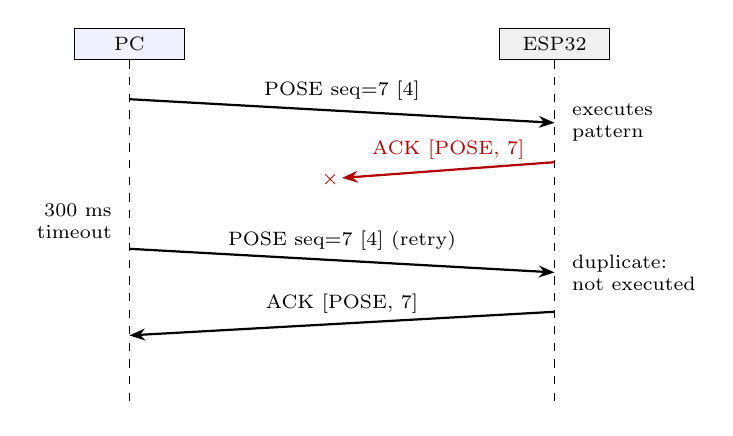
\begin{tikzpicture}[font=\scriptsize, arr/.style={-{Stealth[length=2mm]}, thick}]
			\node[draw, fill=blue!6, minimum width=1.4cm] (pc) at (0,0) {PC};
			\node[draw, fill=gray!12, minimum width=1.4cm] (esp) at (5.4,0) {ESP32};
			\draw[dashed] (pc.south) -- ++(0,-4.4);
			\draw[dashed] (esp.south) -- ++(0,-4.4);
			\draw[arr] (0,-0.7) -- node[above]{POSE seq=7 [4]} (5.4,-1.0);
			\node[anchor=west, align=left] at (5.5,-1.0) {executes\\pattern};
			\draw[arr, red!70!black] (5.4,-1.5) -- node[above]{ACK [POSE, 7]} (2.7,-1.7);
			\node[red!70!black] at (2.55,-1.72) {$\times$};
			\node[anchor=east, align=right] at (-0.1,-2.25) {300 ms\\timeout};
			\draw[arr] (0,-2.6) -- node[above]{POSE seq=7 [4] (retry)} (5.4,-2.9);
			\node[anchor=west, align=left] at (5.5,-2.9) {duplicate:\\not executed};
			\draw[arr] (5.4,-3.4) -- node[above]{ACK [POSE, 7]} (0,-3.7);
		\end{tikzpicture}
		\caption{Retransmission after a lost acknowledgement (rules R2--R4).}
		\label{fig:sequence}
	\end{figure}

	\subsection{Example Frames}

	Table~\ref{tab:examples} lists frames generated by the PC implementation. For instance, the TRACK frame encodes the right hand at $x=0.25$, $y=-0.40$, $|v|=0.472$, and an angle of $302.0^\circ$.

	\begin{table}[!t]
		\centering
		\caption{Example Frames (Hexadecimal)}
		\label{tab:examples}
		\scriptsize

		\setlength{\tabcolsep}{2pt}
		\renewcommand{\arraystretch}{1.05}

		\begin{tabularx}{\columnwidth}{@{}P{1.75cm} c Y@{}}
			\toprule
			Message & SEQ & Frame\\
			\midrule
			PING & 1 & \texttt{A5 02 01 00 C3}\\
			POSE ESCUDO & 2 & \texttt{A5 00 02 01 03 CA}\\
			TRACK & 3 & \texttt{A5 01 03 09 01 FA 00 70 FE D8 01 CC 0B 1E}\\
			MODE (track.) & 4 & \texttt{A5 03 04 01 02 8A}\\
			STOP & 5 & \texttt{A5 04 05 00 EA}\\
			ACK of PING 1 & 0 & \texttt{A5 80 00 02 02 01 6C}\\
			NACK (CRC) & 1 & \texttt{A5 81 01 03 02 04 03 16}\\
			\bottomrule
		\end{tabularx}
	\end{table}


	\section{ESP32 Master Firmware}
	\label{sec:esp32}

	\subsection{Reception and Validation}

	The firmware was developed in the Arduino environment for the ESP32-C3. It advertises the NUS service, and the BLE write callback only copies each received frame into a FreeRTOS queue; the validation and the execution are performed in the main loop, which keeps the BLE task short. Algorithm~\ref{alg:frame} summarizes the processing of each frame.

	\begin{algorithm}[!t]
		\caption{Frame processing in the ESP32}
		\label{alg:frame}
		\begin{algorithmic}[1]
			\Require Received frame $f$ of $n$ bytes
			\If{$n<5$ \textbf{or} $n>19$} \State \Return NACK(\texttt{ERR\_LENGTH}) \EndIf
			\If{$f_0 \neq \texttt{0xA5}$} \State \Return NACK(\texttt{ERR\_SOF}) \EndIf
			\If{$f_3 > 14$ \textbf{or} $n \neq f_3+5$} \State \Return NACK(\texttt{ERR\_LENGTH}) \EndIf
			\If{CRC8$(f_1 \ldots f_{n-2}) \neq f_{n-1}$} \State \Return NACK(\texttt{ERR\_CRC}) \EndIf
			\State Update link watchdog
			\If{TYPE unknown} \State \Return NACK(\texttt{ERR\_UNKNOWN\_TYPE}) \EndIf
			\If{payload invalid} \State \Return NACK(\texttt{ERR\_PAYLOAD}) \EndIf
			\If{\textbf{not} duplicate(TYPE, SEQ)} \State Execute command; store (TYPE, SEQ) \EndIf
			\If{TYPE $\neq$ TRACK} \State \Return ACK(TYPE, SEQ) \EndIf
		\end{algorithmic}
	\end{algorithm}

	\subsection{Motion Patterns}

	To demonstrate the end-to-end operation, each gesture was mapped to a distinct motion of one SOFIA unit with two servomotors driven through a PCA9685 \cite{pca9685,adafruit_pwm}, using the same pin assignment and angle-to-PWM calibration as the servo characterization tests ($-60^\circ$ to $+60^\circ$). Servo channel 0 moves the unit horizontally and channel 1 vertically. The patterns are listed in Table~\ref{tab:patterns}.

	\begin{table}[!t]
		\centering
		\caption{Motion Associated with Each Command}
		\label{tab:patterns}
		\scriptsize

		\setlength{\tabcolsep}{2pt}
		\renewcommand{\arraystretch}{1.05}

		\begin{tabularx}{\columnwidth}{@{}P{2.3cm} P{1.9cm} Y@{}}
			\toprule
			Command & Motion & Detail\\
			\midrule
			POSE 1 INICIO & Circle & 2 turns, radius $35^\circ$\\
			POSE 2 RECARGAR & Square & 2 turns, side $70^\circ$\\
			POSE 3 ESCUDO & X shape & Both diagonals through the center\\
			POSE 4 ATAQUE & Vertical line & 3 strokes of $\pm35^\circ$\\
			POSE 5 FIN & Zigzag & Left to right\\
			TRACK (tracking) & Hand following & $x, y \times 45^\circ$, up to $300^\circ$/s\\
			STOP & Return to center & Interrupts any pattern\\
			\bottomrule
		\end{tabularx}
	\end{table}

	Each pattern is defined as a list of waypoints in normalized coordinates that is scaled to $\pm35^\circ$. Every 20~ms the controller advances the commanded position toward the next waypoint at a constant speed of $120^\circ$/s, converts each angle to PWM counts, and updates the PCA9685 only when the change exceeds $0.1^\circ$. Every pattern ends at the center, and a new gesture interrupts the current pattern. In the safe state, a pattern in progress is allowed to finish, since it ends at the center, while any other motion returns immediately to the center.


	\section{Webots Simulation and Digital Twin}
	\label{sec:webots}

	\subsection{Purpose and Architecture}

	The firmware of Section~\ref{sec:esp32} drives a single unit, while SOFIA is composed of 16. To test the GUI and the communication standard with the complete array, and without depending on the availability of the hardware, a simulation of SOFIA was built in Webots \cite{webots}. Two principles guided its integration. First, the simulation receives \emph{exactly} the same frames as the ESP32, so it also tests the communication standard and not only the motion. Second, the vision processing is not moved to the simulator: the physical camera and MediaPipe remain in the GUI, and the simulation only replaces the robot.

	The resulting architecture is shown in Fig.~\ref{fig:webots}. A new link, \texttt{WebotsLink}, inherits the logic of \texttt{BleLink} (stop-and-wait, retransmission with the same SEQ, TRACK at 20~Hz, and heartbeat) and only replaces the transport. It runs in its own thread, like the BLE link. The overhead virtual camera uses a separate controller and a separate socket, so a failure of the camera channel does not affect the commands.

	\begin{figure}[!t]
		\centering
		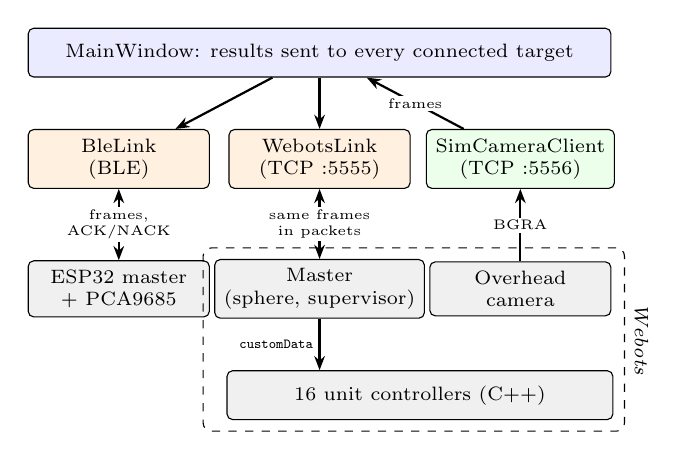
\begin{tikzpicture}[
			font=\scriptsize,
			box/.style={draw, rounded corners=2pt, align=center, minimum width=2.3cm, minimum height=0.62cm, fill=white},
			grp/.style={draw, dashed, rounded corners=3pt, inner sep=4pt},
			arr/.style={-{Stealth[length=1.8mm]}, thick},
			lbl/.style={font=\tiny, align=center, fill=white, inner sep=1pt}
			]
			% GUI side
			\node[box, fill=blue!8, minimum width=7.4cm] (gui) at (0,0) {MainWindow: results sent to every connected target};
			\node[box, fill=orange!12] (ble) at (-2.55,-1.35) {BleLink\\(BLE)};
			\node[box, fill=orange!12] (sim) at (0,-1.35) {WebotsLink\\(TCP :5555)};
			\node[box, fill=green!8] (cam) at (2.55,-1.35) {SimCameraClient\\(TCP :5556)};
			% Targets
			\node[box, fill=gray!12] (esp) at (-2.55,-3.0) {ESP32 master\\+ PCA9685};
			\node[box, fill=gray!12] (mae) at (0,-3.0) {Master\\(sphere, supervisor)};
			\node[box, fill=gray!12] (ccam) at (2.55,-3.0) {Overhead\\camera};
			\node[box, fill=gray!12, minimum width=4.9cm] (pan) at (1.275,-4.35) {16 unit controllers (C++)};

			\node[grp, fit=(mae)(ccam)(pan), label={[font=\scriptsize\itshape]right:\rotatebox{-90}{Webots}}] {};

			\draw[arr] (gui) -- (ble);
			\draw[arr] (gui) -- (sim);
			\draw[arr] (cam) -- node[lbl]{frames} (gui);
			\draw[{Stealth[length=1.8mm]}-{Stealth[length=1.8mm]}, thick] (ble) -- node[lbl]{frames,\\ACK/NACK} (esp);
			\draw[{Stealth[length=1.8mm]}-{Stealth[length=1.8mm]}, thick] (sim) -- node[lbl]{same frames\\in packets} (mae);
			\draw[arr] (ccam) -- node[lbl]{BGRA} (cam);
			\draw[arr] (mae) -- node[lbl, left=1pt]{\texttt{customData}} (mae |- pan.north);
		\end{tikzpicture}
		\caption{Integration of the Webots simulation with the GUI. The command link and the camera stream use independent threads and sockets; when both the ESP32 and Webots are connected, every command is sent to both (digital twin).}
		\label{fig:webots}
	\end{figure}

	\subsection{Transport over TCP}

	BLE transfers packets, whereas TCP transfers a stream of bytes. To preserve the rule that one BLE write carries exactly one frame, each frame is sent over TCP preceded by one byte with its length, $[N][\text{frame of } N \text{ bytes}]$. The master extracts the frame and validates it with the same procedure as Algorithm~\ref{alg:frame}. The PC side of \texttt{protocol.py} is reused without changes: the simulated master loads the same file, so the frame format, the CRC-8, and the error codes cannot diverge between the robot and the simulation.

	A local socket delivers every frame in less than 1~ms and without errors, which would hide the retransmission rules. Therefore, the GUI includes an optional channel emulator for the Webots link, with the parameters of Table~\ref{tab:channel}. With it, the retransmissions, the duplicate rejection, and the NACK with \texttt{ERR\_CRC} appear in the event log as they would over BLE.

	\begin{table}[!t]
		\centering
		\caption{Parameters of the Optional Channel Emulator}
		\label{tab:channel}
		\scriptsize

		\setlength{\tabcolsep}{2pt}
		\renewcommand{\arraystretch}{1.05}

		\begin{tabularx}{\columnwidth}{@{}P{3.0cm} Y@{}}
			\toprule
			Parameter & Value\\
			\midrule
			Delay per direction & $30 \pm 10$~ms\\
			Frame loss & 3\,\%\\
			Corrupted byte (detected by CRC) & 2\,\%\\
			\bottomrule
		\end{tabularx}
	\end{table}

	\subsection{Simulated Master Controller}

	The master is a Python supervisor controller attached to a sphere that represents the target of the array. It reproduces the behavior of the firmware: it answers ACK or NACK, does not execute a repeated command with the same TYPE and SEQ within 1~s (rule R4), and enters the safe state after 3~s without valid frames or when the GUI disconnects (rule R8). Its response to each command is summarized in Table~\ref{tab:simcommands}.

	\begin{table}[!t]
		\centering
		\caption{Response of the Simulation to Each Command}
		\label{tab:simcommands}
		\scriptsize

		\setlength{\tabcolsep}{2pt}
		\renewcommand{\arraystretch}{1.05}

		\begin{tabularx}{\columnwidth}{@{}P{1.9cm} Y@{}}
			\toprule
			Command & Effect in the simulation\\
			\midrule
			TRACK (tracking) & The sphere moves to the hand position, up to 0.30~m from the center, and the 16 units point at it\\
			POSE & The 16 units execute the pattern of the gesture (Table~\ref{tab:simpatterns})\\
			MODE & Forwarded to the units; entering or leaving tracking resets the sphere\\
			STOP / safe state & Units return to the center; any pattern is canceled\\
			No GUI connected & Game mode; units remain at the center\\
			\bottomrule
		\end{tabularx}
	\end{table}

	The master does not move the units directly. It writes a short text command into its own \texttt{customData} field, \texttt{M<mode> IDLE}, \texttt{M<mode> TRACK}, or \texttt{M<mode> POSE <id> <t\textsubscript{0}>}, and the 16 unit controllers read it at every simulation step. The field $t_0$ is the simulation time at which the gesture was received; since all the units compute their pattern from the same $t_0$, the 16 units move in synchronism without additional messages. The units follow the sphere only in tracking mode; in game and test modes the sphere is hidden and the units stay at the center, except while executing a pattern.

	\subsection{Unit Controllers}

	Each simulated unit has two rotational joints with mechanical limits of $\pm30^\circ$, and its controller is written in C++. In tracking mode, the controller computes the unit vector $\mathbf{v}=(v_x,v_y,v_z)$ from the pivot of the unit to the sphere and obtains the joint angles as
	\begin{equation}
		\theta_1 = \operatorname{atan2}(-v_y,\, v_z), \qquad \theta_2 = \arcsin(v_x).
		\label{eq:ik}
	\end{equation}
	Every step of 8~ms, the commanded angles are limited to $\pm27.5^\circ$ and approached gradually, advancing 15\,\% of the remaining error with a maximum of $0.15$~rad per step, which avoids abrupt jumps of the physics engine.

	The patterns of the simulation (Table~\ref{tab:simpatterns}) were designed to be recognizable on the array of 16 units when observed from the overhead camera, so they differ from the single-unit patterns of Table~\ref{tab:patterns}. Each pattern is a list of waypoints scaled to an amplitude of $0.35$~rad ($\approx20^\circ$) and traversed at constant speed; RECARGAR is the only pattern in which the units do not move in unison.

	\begin{table}[!t]
		\centering
		\caption{Motion Patterns of the 16-Unit Simulation}
		\label{tab:simpatterns}
		\scriptsize

		\setlength{\tabcolsep}{2pt}
		\renewcommand{\arraystretch}{1.05}

		\begin{tabularx}{\columnwidth}{@{}P{1.7cm} Y P{0.9cm}@{}}
			\toprule
			Gesture & Motion (seen from the overhead camera) & Duration\\
			\midrule
			1 INICIO & Up and down, all units in unison & 1.6~s\\
			2 RECARGAR & Loading circle: the 12 border units tilt outward one after another, 2 clockwise turns & 2.4~s\\
			3 ESCUDO & Rhombus, all units in unison & 3.1~s\\
			4 ATAQUE & L shape, all units in unison & 1.9~s\\
			5 FIN & Left and right (farewell), all units in unison & 2.3~s\\
			\bottomrule
		\end{tabularx}
	\end{table}

	\subsection{Virtual Camera}

	An overhead camera of $320\times320$ pixels captures the array every 64~ms ($\approx15$~frames per second). Its controller only transmits images: each one is preceded by a header with the identifier \texttt{SOFC}, the width and height (16 bits each), and the size (32 bits), followed by the BGRA pixels. In the GUI, a dedicated \texttt{QThread} receives the images and displays them next to the live video, so the operator can see, in the same window, the gesture performed in front of the physical camera and the response of the simulated array.

	\subsection{Operating Configurations and Digital Twin}

	The GUI sends each result to every connected target, which yields the three configurations of Table~\ref{tab:configs}. When both are connected, every POSE, TRACK, MODE, and STOP frame is transmitted to the physical robot and to the simulation at the same time, and the simulation operates as a digital twin. The event log labels each message with its target, \texttt{[ESP32]} or \texttt{[Webots]}, together with the time of its acknowledgement, so the responses of both can be compared.

	\begin{table}[!t]
		\centering
		\caption{Operating Configurations}
		\label{tab:configs}
		\scriptsize

		\setlength{\tabcolsep}{2pt}
		\renewcommand{\arraystretch}{1.05}

		\begin{tabularx}{\columnwidth}{@{}P{1.9cm} Y@{}}
			\toprule
			Connected & Use\\
			\midrule
			Webots only & Development and testing of the GUI, the protocol, and the patterns without hardware\\
			ESP32 only & Operation of the physical robot\\
			ESP32 and Webots & Digital twin: the same commands drive the robot and the simulation\\
			\bottomrule
		\end{tabularx}
	\end{table}


	\section{Verification}
	\label{sec:verification}

	The implementation was verified at the software level and in the Webots simulation; the tests are summarized in Table~\ref{tab:verification}. The GUI was executed with the camera and the detection pipeline replaced by stubs, and the controls were applied in sequence. The BLE link was tested against a simulated ESP32 that reproduces the validation and duplicate-rejection rules of the firmware. The CRC-8 of the firmware was compiled and compared with the PC implementation, and the complete firmware was compiled on a PC with simulated Arduino, BLE, and PCA9685 interfaces, injecting the same frames that the PC sends and recording the PWM commands of each servo.

	\begin{table}[!t]
		\centering
		\caption{Verification Results}
		\label{tab:verification}
		\scriptsize

		\setlength{\tabcolsep}{2pt}
		\renewcommand{\arraystretch}{1.05}

		\begin{tabularx}{\columnwidth}{@{}P{2.4cm} Y P{1.2cm}@{}}
			\toprule
			Test & Observed result & Status\\
			\midrule
			Controls of the thread & States: loading, running, paused, running, stopped; no frames emitted while paused & \status{Passed}\\
			CRC-8 (PC and ESP32) & Check value \texttt{0xF4} and identical CRC for all example frames & \status{Passed}\\
			Command with ACK & PING and POSE acknowledged & \status{Passed}\\
			Lost ACK (R3, R4) & Retransmitted with the same SEQ; executed once & \status{Passed}\\
			No response (R3) & Three attempts, then reported as failed & \status{Passed}\\
			Invalid payload & NACK \texttt{ERR\_PAYLOAD}, no retransmission & \status{Passed}\\
			TRACK rate (R6) & 10 frames in 0.5~s (20~Hz) & \status{Passed}\\
			Heartbeat (R7) & PING sent after 1~s without traffic & \status{Passed}\\
			Motion patterns & Five distinct trajectories, all ending at the center (Fig.~\ref{fig:trajectories}) & \status{Passed}\\
			Webots link & Frames acknowledged by the simulated master; each gesture executes its pattern on the 16 units & \status{Passed}\\
			Modes in Webots & Units follow the sphere only in tracking mode and stay at the center in game and test modes & \status{Passed}\\
			Virtual camera & Overhead view displayed in the GUI next to the live video & \status{Passed}\\
			Digital twin & Same commands sent to the ESP32 and to Webots & \status{Pending}\\
			Physical hardware & BLE link established; frames acknowledged and the unit moved as expected (visual inspection, no measurements) & \status{Passed}\\
			Hardware metrics & Latency and positioning accuracy on the real unit & \status{Pending}\\
			\bottomrule
		\end{tabularx}
	\end{table}

	Fig.~\ref{fig:trajectories} shows the trajectories obtained from the simulated firmware, computed by converting the PWM counts sent to each servo back into angles. The five gestures produce distinguishable trajectories, and the tracking mode follows the commanded hand position. The staircase appearance corresponds to the resolution of the PCA9685 with the adopted calibration, in which 160 counts cover $120^\circ$ ($\approx0.75^\circ$ per count). The simulated durations of the patterns range from 2.4~s (FIN) to 5.6~s (RECARGAR).

	\begin{figure*}[!t]
		\centering
		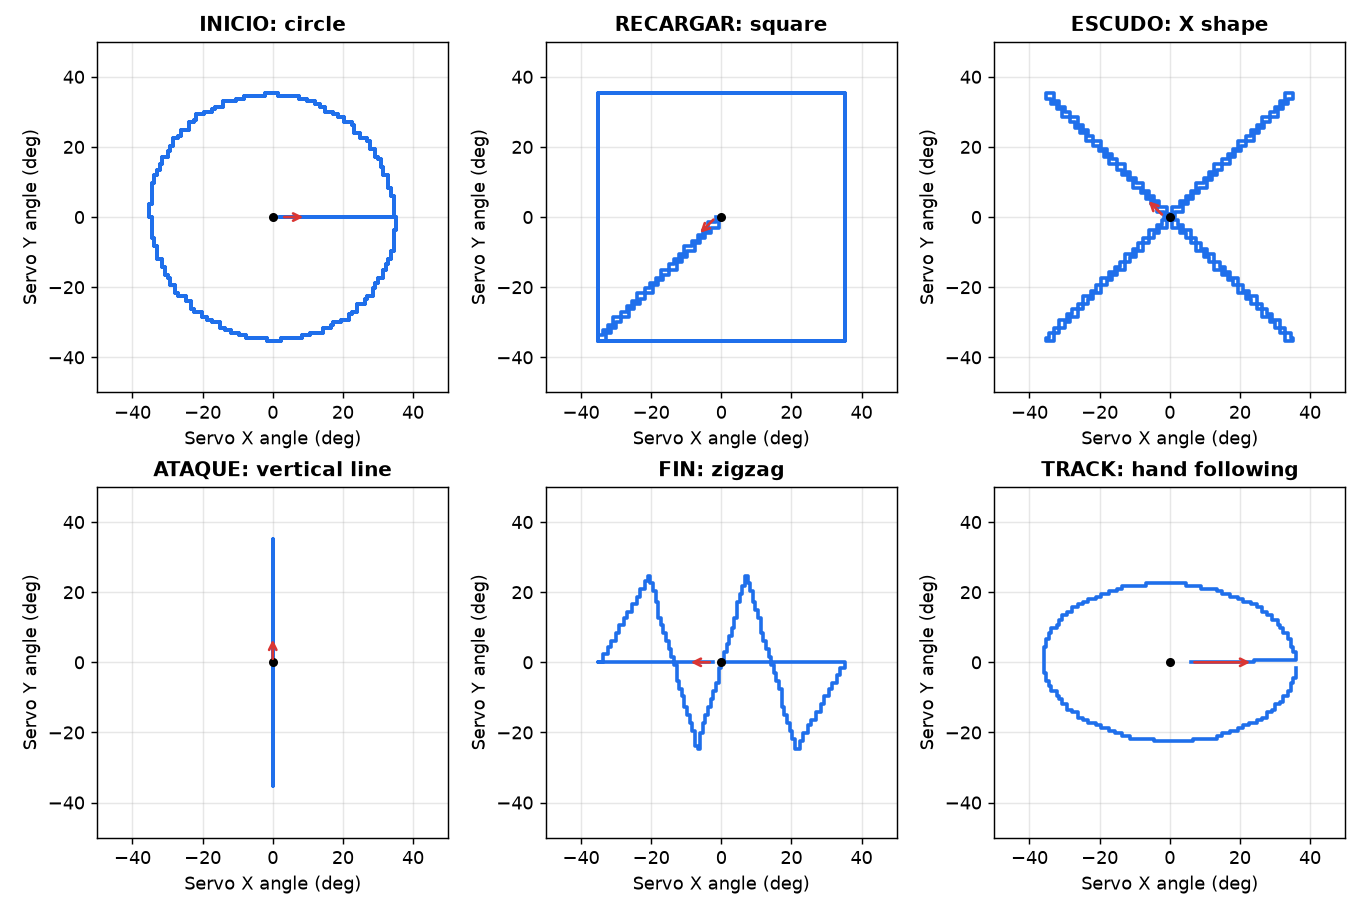
\includegraphics[width=0.85\textwidth]{figures/pattern_trajectories}
		\caption{Trajectories of the unit generated by the simulated ESP32 firmware for each command. The black dot marks the center and the red arrow the initial direction.}
		\label{fig:trajectories}
	\end{figure*}

	Finally, a preliminary functional test was performed on the physical hardware. The firmware was loaded on the ESP32-C3, which was connected to one unit through the PCA9685, and the PC established the BLE link with it. The commands sent from the PC were acknowledged, and the unit executed the expected motions within the expected parameters. This test was based on visual inspection; no quantitative measurements of latency or positioning accuracy were taken, so the characterization of the hardware remains pending.


	\section{Conclusions}
	\label{sec:conclusions}

	A GUI was developed for the SOFIA vision system using PySide6. Separating the interface, the video processing, and the BLE communication into three threads keeps the interface responsive, and the start, pause, resume, and stop controls act directly on the processing thread through a mutex and a wait condition. A communication standard was defined to transmit the recognized gestures and the hand position from the PC to the ESP32 master; its frame structure, CRC-8 checksum, acknowledgements, error codes, and retransmission and supervision rules address lost frames, corrupted frames, and loss of the link. An ESP32 firmware that receives, validates, and acknowledges the frames was implemented and associated with five distinct motion patterns of a two-degree-of-freedom unit. In addition, a Webots simulation of the 16-unit array was integrated with the GUI through a simulated master that receives the same frames and applies the same rules as the firmware, so the communication standard, the modes, and the motion patterns can be tested on the complete array without hardware, and the simulation can run alongside the physical robot as a digital twin. The software verification confirmed the expected behavior of the controls, the protocol rules, and the motion patterns, and a preliminary test on the physical ESP32 and one unit confirmed the BLE link and the servo motion. Future work includes the quantitative characterization of the hardware, the measurement of the end-to-end latency from gesture to motion and of the delay between the robot and its digital twin, and the extension of the motion commands of the firmware to the 16 modules of SOFIA, using the patterns validated in the simulation.



	\balance

	\bibliographystyle{IEEEtran}
	\bibliography{bibliography}

\end{document}
